\section{Problem Statement}

Different cloud service companies ensure data availability and safety. However, they have ``terms of use'' that allow the company to edit, modify, access, delete, view, and analyze your content. And that to provide the best possible service to the client, create an advertisement, manipulate it in some way to generate income, or use it for their purpose or analysis. \\

However, storing sensitive data only on local machines or drives can sometimes be very lamenting because once they are lost or destroyed by any other means, you cannot make a recovery. Moreover, most of the personal accounts of cloud storage also do not cover the insurance of data or take responsibility in case of data loss due to catastrophic failure. So, relying on data stored on your local machine only or the cloud storage is just not always safe and genuine. \\

As for the protocol itself, when you want to visit a website today, your browser (client) sends a request to the servers (host) that ``serve'' up that website, even when those servers are across the globe from your current location. This is location-based addressing, and it uses \gls{ip} addresses to show your location. That process eats \gls{bandwidth}, and thus costs us a lot of money and time. On top of that, \gls{http} downloads a file from a single server at a time, which is way worse than getting multiple pieces of that file from multiple computers. It also allows for powerful entities to block access to certain locations, like Turkey did with the Wikipedia servers in 2017.

\namedfigure
{!htbp}
{img:httpVIpfs}
{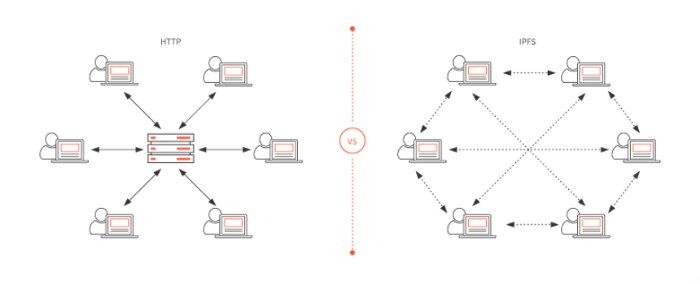
\includegraphics[width=0.9\textwidth]{http-vs-ipfs.png}}
{HTTP location-based addressing vs IPFS content-based addressing.}

